\documentclass[11pt]{article}
\usepackage{setspace}
\setstretch{1}
\usepackage{amsmath,amssymb, amsthm}
\usepackage{graphicx}
\usepackage{bm}
\usepackage[hang, flushmargin]{footmisc}
\usepackage[colorlinks=true]{hyperref}
\usepackage[nameinlink]{cleveref}
\usepackage{footnotebackref}
\usepackage{url}
\usepackage{listings}
\usepackage[most]{tcolorbox}
\usepackage{inconsolata}
\usepackage[papersize={8.5in,11in}, margin=1in]{geometry}
\usepackage{float}
\usepackage{caption}
\usepackage{esint}
\usepackage{url}
\usepackage{enumitem}
\usepackage{subfig}
\usepackage{wasysym}
\newcommand{\ilc}{\texttt}
\newcommand{\p}{\partial}
\usepackage{etoolbox}
\usepackage{algorithm}
\usepackage{changepage}
% \usepackage{algorithmic}
\usepackage[noend]{algpseudocode}
\usepackage{tikz}


\usetikzlibrary{matrix,positioning,arrows.meta,arrows}
\patchcmd{\thebibliography}{\section*{\refname}}{}{}{}
% \PassOptionsToPackage{hyphens}{url}\usepackage{hyperref}

\providecommand{\myceil}[1]{\left \lceil #1 \right \rceil }
\providecommand{\myfloor}[1]{\left \lfloor #1 \right \rfloor }

\definecolor{dkgreen}{rgb}{0,0.6,0}
\definecolor{gray}{rgb}{0.5,0.5,0.5}
\definecolor{mauve}{rgb}{0.58,0,0.82}

\lstset{frame=tb,
  language=Python,
  aboveskip=3mm,
  belowskip=3mm,
  showstringspaces=false,
  columns=flexible,
  basicstyle={\small\ttfamily},
  numbers=none,
  numberstyle=\tiny\color{gray},
  keywordstyle=\color{blue},
  commentstyle=\color{dkgreen},
  stringstyle=\color{mauve},
  breaklines=true,
  breakatwhitespace=true,
  tabsize=3
}

\begin{document}


\title{\textbf{CSDS 491: Assignment 1}}

\author{Shaochen (Henry) ZHONG, ilc{sxz517@case.edu}}

\date{Due and submitted on 02/22/2021 \\ Spring 2021, Dr. Lewicki}
\maketitle


% We've received some common questions for A1.  Here are some hints to help you go in the right direction.
%
% Q2.2: You need only prove there is a logical gap that would require an additional assumption.
%
% Q4: It is helpful to use the conjugate prior as shown in lecture.  The  normalization factor for the posterior then has the same form as the prior (but with different arguments).
%
% Q5: Remember that the data consists of event times, and the posterior is in terms of the Poisson rate parameter lambda given the number of observed data events in a given duration from 0 to T.  You only need a single Poisson likelihood combined with the prior to get the posterior.
%
% Exploration: The terms discrete and continuous refer to the variables in the model.  See the rubric for the grading criteria. Try to make your inference problems simple models of real-world situations, rather than just numerical examples.


\section*{Q1}


\subsection*{1.1.}

\begin{align*}
    p(x, y  \mid  z) &= \frac{p(x, y, z)}{p(x)} \\
    &= \frac{p(x, y, z) \cdot p(x, z)}{p(x) \cdot p(x, z)} \\
    &= \frac{p(x, z)}{p(z)} \cdot \frac{p(x, y, z)}{p(x, z)} \\\
    &= p(x  \mid  z) p(y  \mid  x, z)
\end{align*}

\subsection*{1.2.}


\begin{align*}
    p(x  \mid  y, z) &= \frac{p(x, y, z)}{p(y, z)} \\
    &= \frac{\frac{p(x, y, z)}{p(z)}}{\frac{p(y, z)}{p(z)}} = \frac{\frac{p(x, y, z)}{p(x, z)}\frac{p(x, z)}{p(z)}}{p(y  \mid  z)} \\
    &= \frac{p(y  \mid  x, z) p(x  \mid  z)}{p(y  \mid  z)}
\end{align*}


\section*{Q1}
\subsection*{2.1.}

Assume $a = \{1, 2, 3 \}$, $b = \{1, 4 \}$, $c = \{1, 2, 6 \}$ from a set of $\{1, 2, 3, 4, 5, 6\}$, we have:

\begin{align*}
    p(a, b) &= \frac{\{1\}}{\{1, 2, 3, 4, 5, 6\}} = \frac{1}{6} = p(a)p(b) = \frac{1}{2} \cdot \frac{1}{3} \Longrightarrow a \bot b \\
    p(b, c) &= \frac{\{1\}}{\{1, 2, 3, 4, 5, 6\}} = \frac{1}{6} = p(b)p(c) = \frac{1}{2} \cdot \frac{1}{3} \Longrightarrow b \bot c \\
    p(a, c) &= \frac{\{1, 2\}}{\{1, 2, 3, 4, 5, 6\}} = \frac{1}{3} \\
    p(a)p(c) &= \frac{1}{2}\cdot \frac{1}{2} = \frac{1}{4} \\
    \Longrightarrow p(a, c) &\neq p(a)p(c)
\end{align*}

This suggests $a \bot b \wedge b \bot c \not \Rightarrow a \bot c$. For an example, we may have

\begin{itemize}
    \item \textbf{a}: Rainning tomorrow.
    \item \textbf{b}: Had pasta as dinner today.
    \item \textbf{c}: Not rainning tomorrow.
\end{itemize}

By common sense we know that $a \bot b \wedge b \bot c$ holds true, but we can't have $a \bot c$ as it must be one way or another in terms rainning tomorrow or not.

\subsection*{2.2.}

Assume $a \bot b  \mid  c$, we have:
\begin{align*}
    p(a, (b  \mid  c)) &= p(a) p(b  \mid  c)\\
    &= p(a)\frac{p(b, c)}{p(c)}
\end{align*}

To have $a \bot b$, we must show $p(a, b) = p(a)p(b)$. The only way to convert the above equation to such format is to assume $b \bot c$ so that we can have:


\begin{align*}
    p(a, (b  \mid  c)) &= p(a)\frac{p(b, c)}{p(c)} \\
    p(a, b) &= p(a) \frac{p(b)p(c)}{p(c)} \\
    p(a, b) &= p(a)p(b)
\end{align*}

But $b \bot c$ is an assumption which cannot be guaranteed.

\section*{Q3}

Please refer to \ilc{code/q3.py} for code.

\subsection*{3.1.}

\ilc{0.7281553398058251}

\subsection*{3.2.}
\ilc{0.9765625}

I am aming to have $p(B  \mid  K) > 0.9$, thus I will need to lower the possibility of scenarios where the butler is not the killer. I found $p(K  \mid  B = F, M = F)$ and $p(K  \mid  B = F, M = T)$ to be more ``explainable'' as for the former we may simply say the inspector had more on-scence info indicating the killer is very likely to be still in the house; for the latter we may also just let the scence implies that the victim is strong and tall but the maid is petite with no sign of combat -- thus lowering the possibility of $M=T$ along.

\subsection*{3.3.}

\begin{align*}
    p(M  \mid  K) &= \sum_{b}p(b,M \mid K) =\sum_{b}\frac{p(b,M,K)}{p(K)} \\
    &= \frac{\sum_{b}p(K \mid b,M)p(b,M)}{\sum_{b,m}p(K \mid b,m)p(b,m)} = \frac{p(M)\sum_{b}p(K \mid b,M)p(b)}{\sum_{m}p(m)\sum_{b}p(K \mid b,m)p(b)}
\end{align*}

\subsection*{3.4.}

With the setup proposed by the textbook, we have $p(M \mid K)$ being  \ilc{0.06796116504854369}; with the setup defined by me, we have $p(M \mid K)$ being \ilc{0.05208333333333333}.\newline

The main contributing factor is $p(K  \mid  B = F, M = T)$, as we have lowered it in the second setup, we directly decrease the chances of the maid being the murder and thus potentially lowered $p(M \mid K)$. We may also confirm this guessing by calculating only with the lowered $p(K  \mid  B = F, M = F)$ and only with the lowered $p(K  \mid  B = F, M = T)$. We got \ilc{0.08771929824561403} with only the lowered $p(K  \mid  B = F, M = F)$ and \ilc{0.04} with only the lowered $p(K  \mid  B = F, M = T)$ -- suggesting that knowing the maid is very unlikely to be the murder herslef ($\downarrow p(K  \mid  B = F, M = T)$) has more of an impact on $p(M \mid K)$ than knowing the murder is more likely to be between bulter and maid ($\downarrow p(K  \mid  B = F, M = F)$).


\section*{Q4}

Please refer to \ilc{code/q4.py} for complete code.

\subsection*{4.1.}

\begin{lstlisting}
    def p_theta__beta(theta, y, n, alpha, beta):
        return stats.beta.pdf(theta, alpha + y, beta + n - y)
\end{lstlisting}

\subsection*{4.2.}

\begin{figure}[H]
\minipage{0.4\textwidth}
  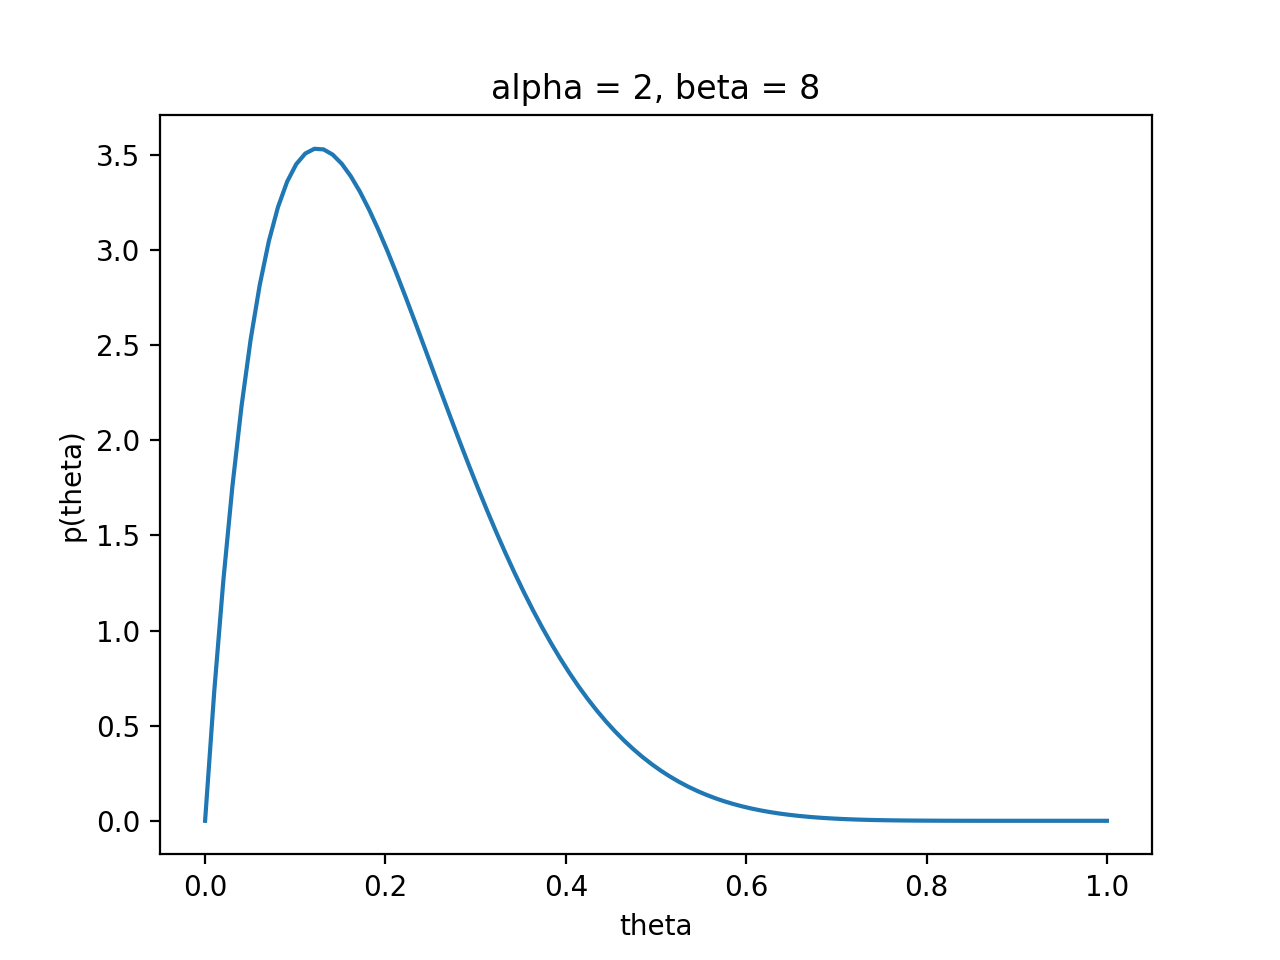
\includegraphics[width=\linewidth]{{fig/q4.2_1}.png}
  \caption*{Biased coin, more likely tail.}
\endminipage\hfill
\minipage{0.4\textwidth}
  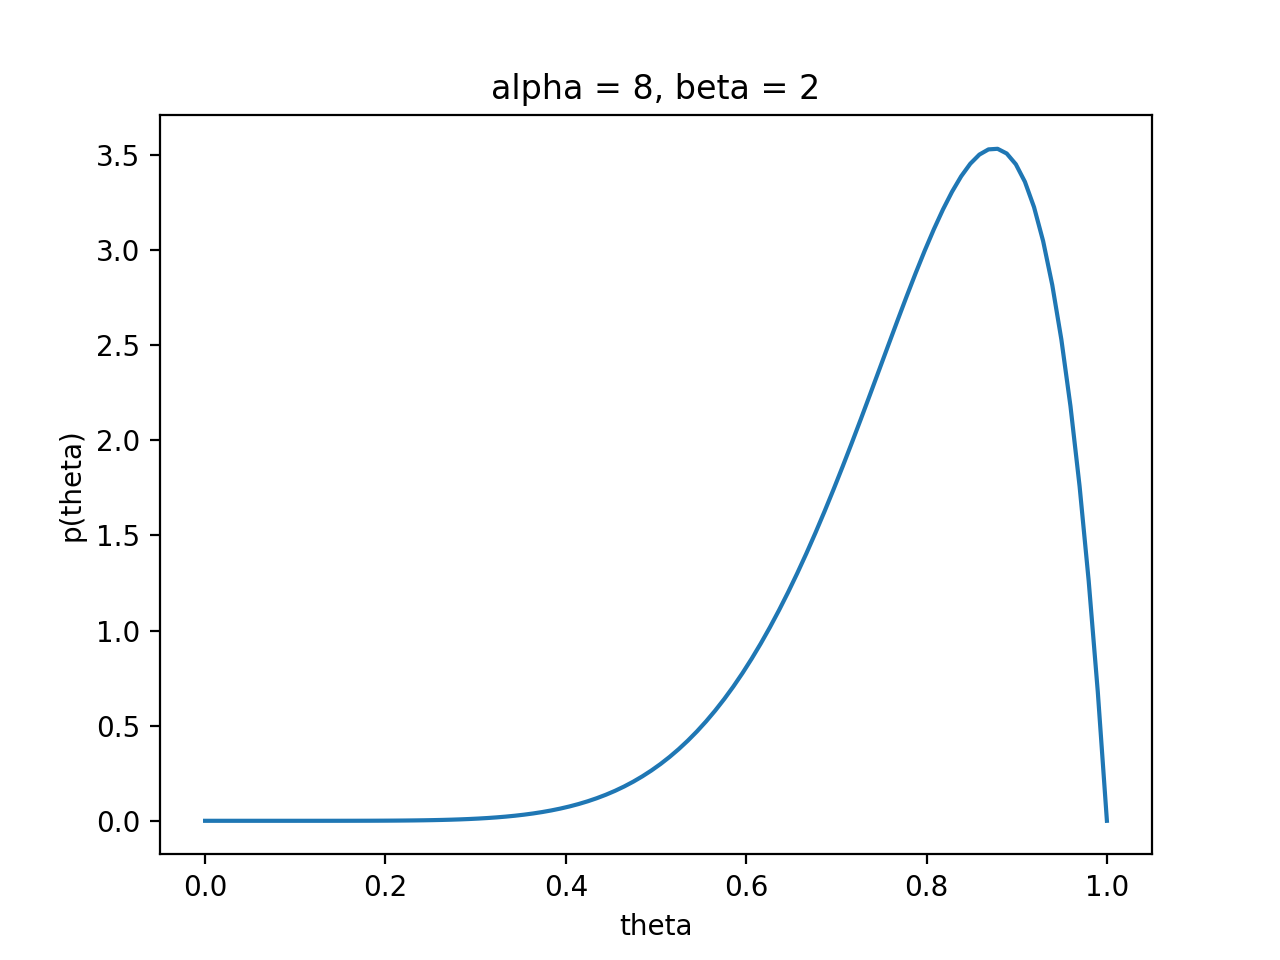
\includegraphics[width=\linewidth]{{fig/q4.2_2}.png}
  \caption*{Biased coin, more likely head.}
\endminipage
\end{figure}

Alternatively we may have it on the same plot with $\alpha < 1, \beta < 1$:
\begin{figure}[H]
    \centering
    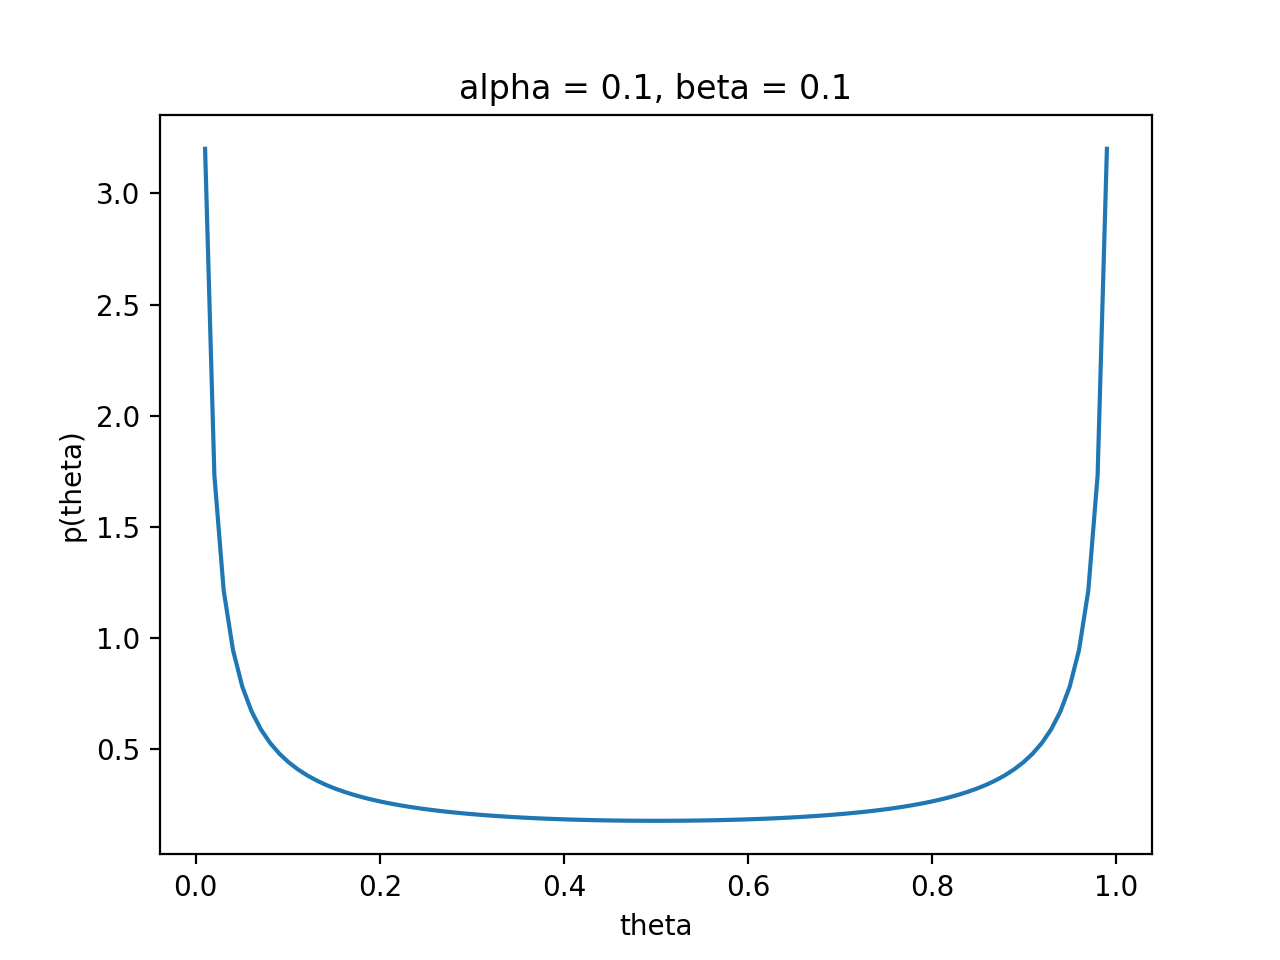
\includegraphics[width=0.4\linewidth]{{fig/q4.2_1_alt}.png}\
    \caption*{Biased coin (either way).}
\end{figure}



\begin{figure}[H]
\minipage{0.4\textwidth}
  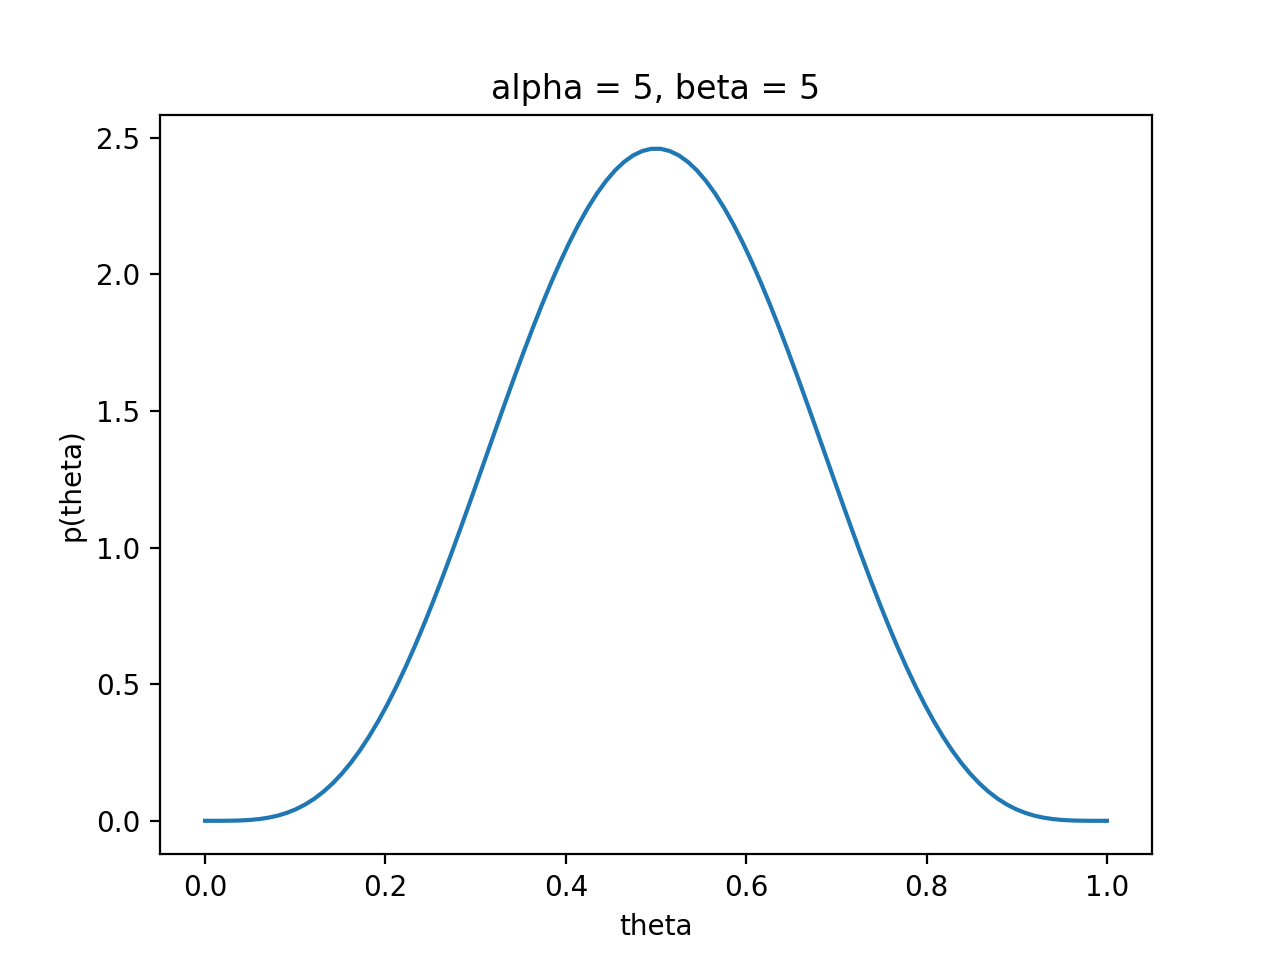
\includegraphics[width=\linewidth]{{fig/q4.2_3}.png}
  \caption*{Unbiased coin}
\endminipage\hfill
\minipage{0.4\textwidth}
    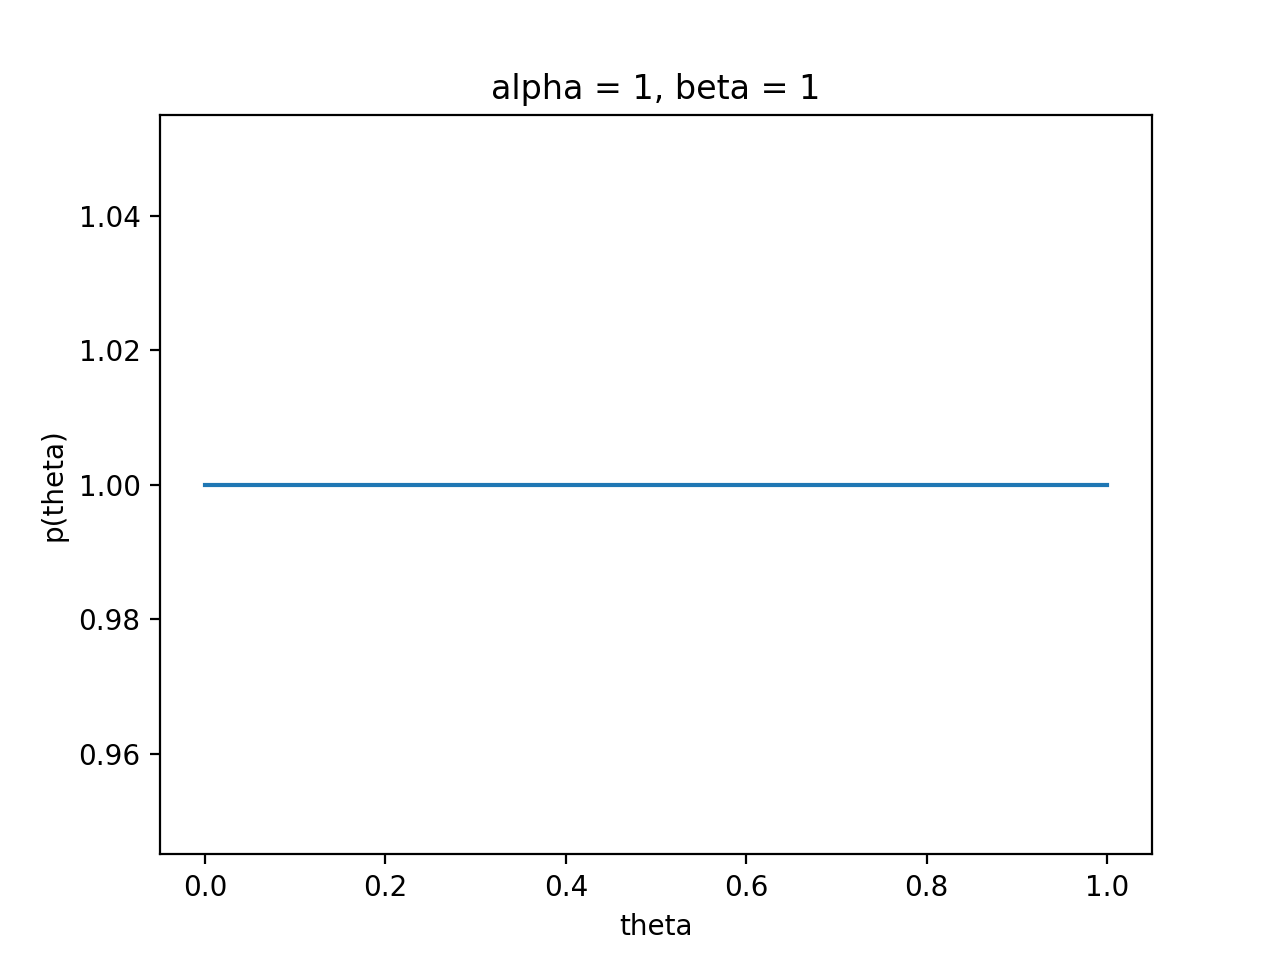
\includegraphics[width=\linewidth]{{fig/q4.2_4}.png}
    \caption*{No info coin}
\endminipage
\end{figure}



\subsection*{4.3.}

\begin{figure}[H]
\minipage{0.3\textwidth}
  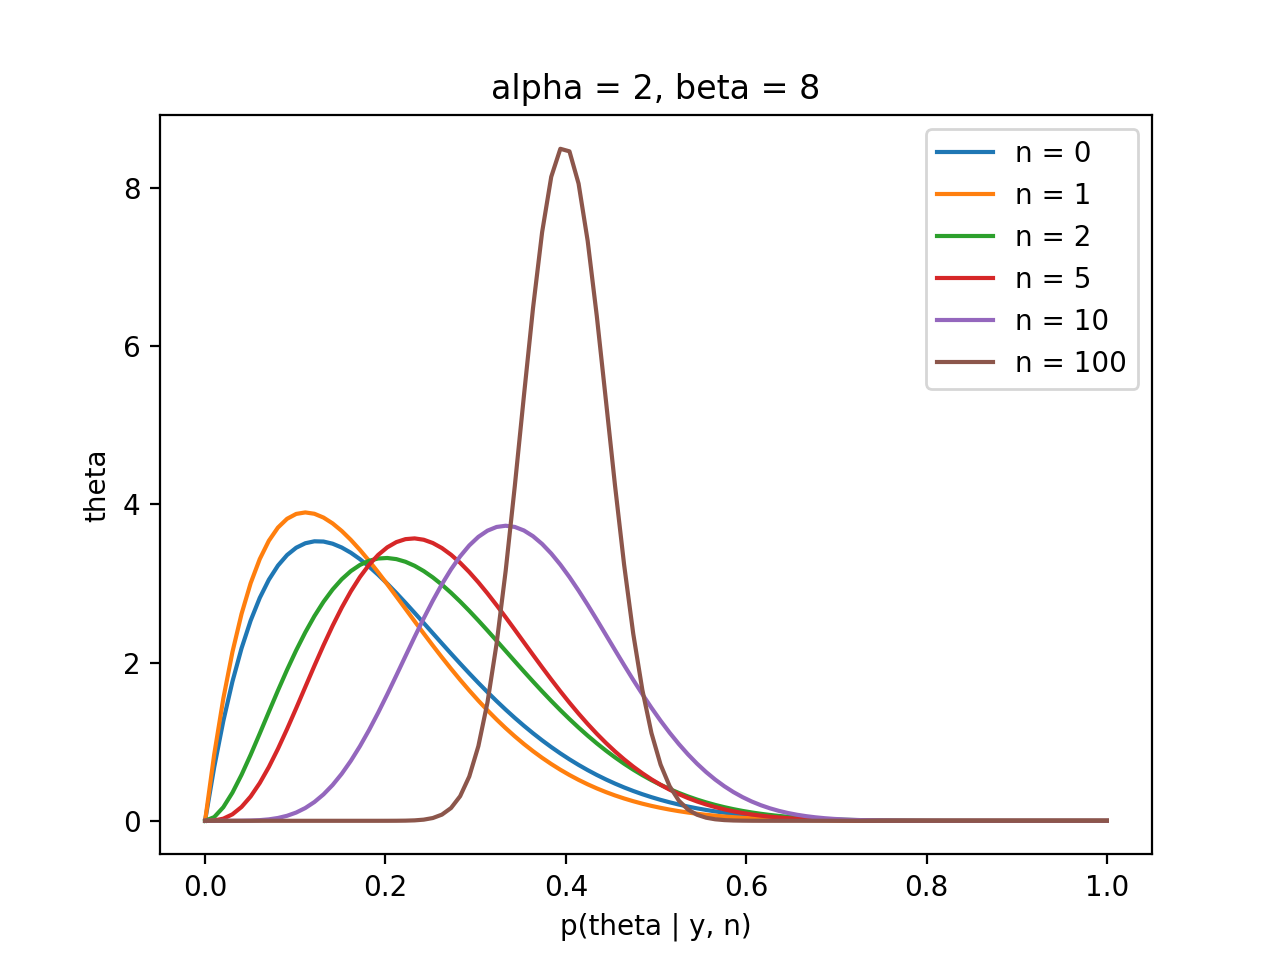
\includegraphics[width=\linewidth]{{fig/q4.3_1}.png}
  \caption*{Biased coin, more likely tail.}
\endminipage\hfill
\minipage{0.3\textwidth}
  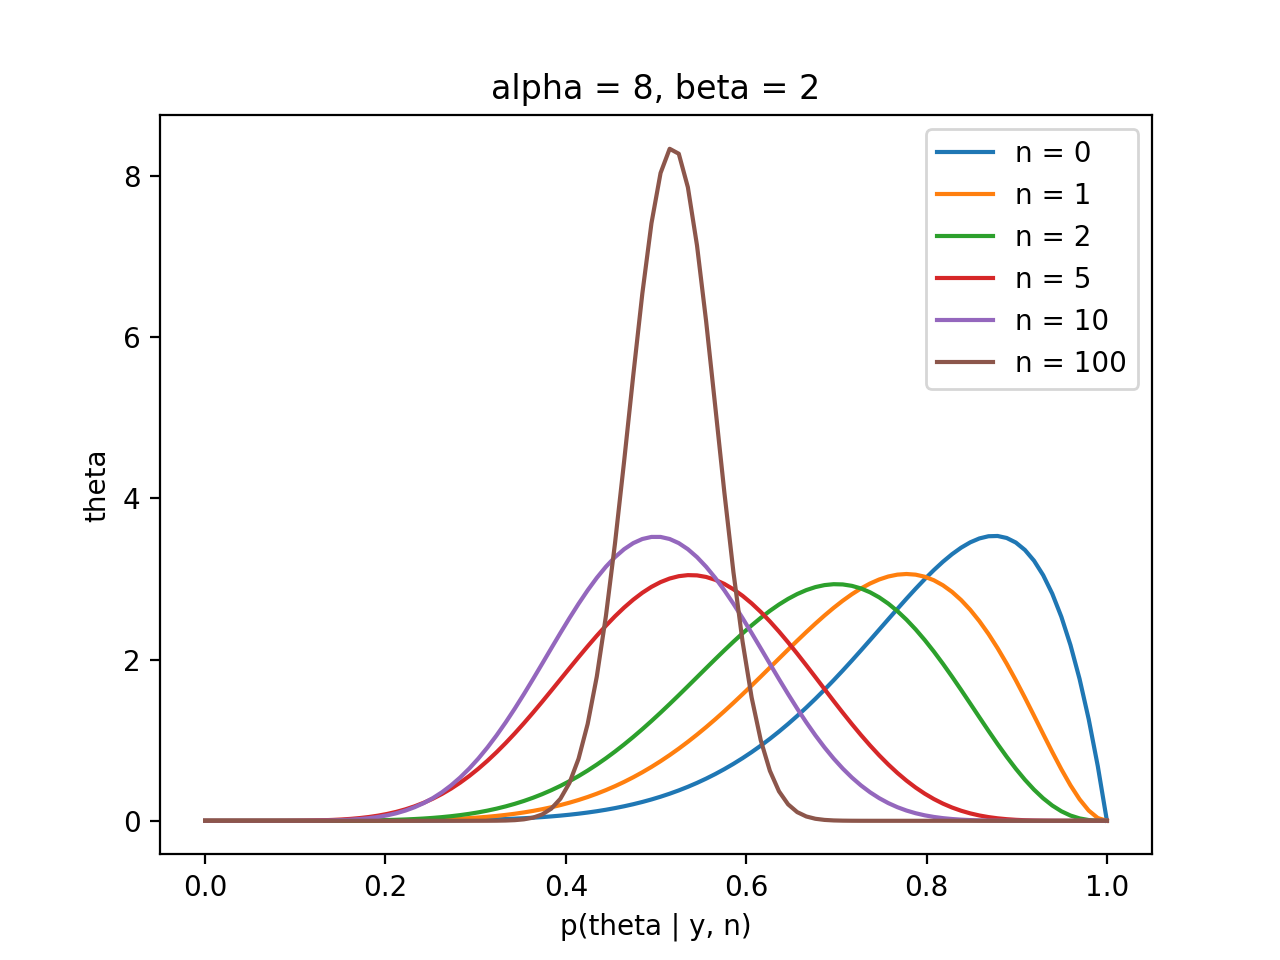
\includegraphics[width=\linewidth]{{fig/q4.3_2}.png}
  \caption*{Biased coin, more likely head.}
\endminipage\hfill
\minipage{0.3\textwidth}
  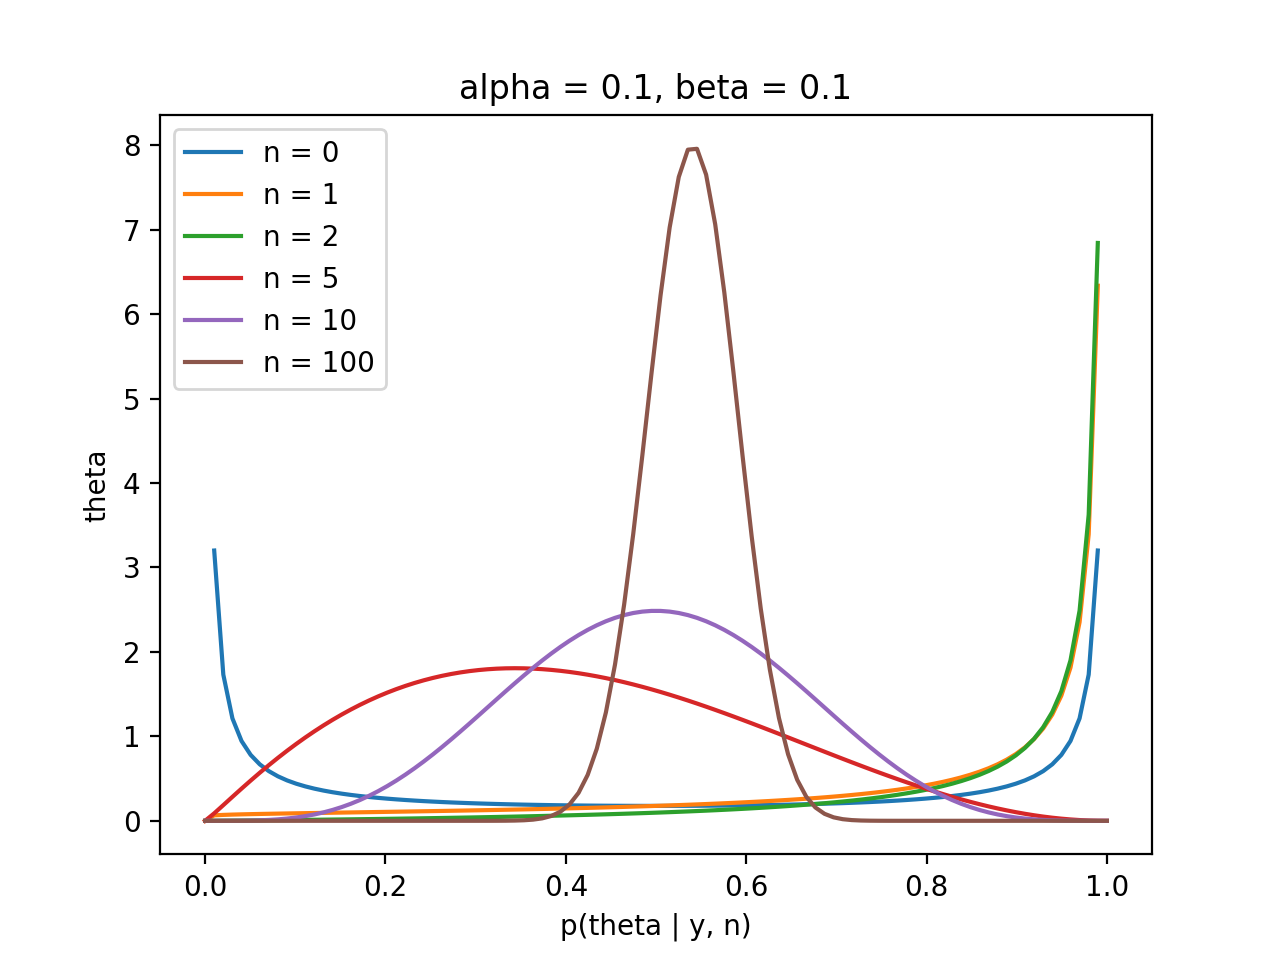
\includegraphics[width=\linewidth]{{fig/q4.3_1_alt}.png}
  \caption*{Biased coin (either way).}
\endminipage
\end{figure}

\begin{figure}[H]
\minipage{0.4\textwidth}
  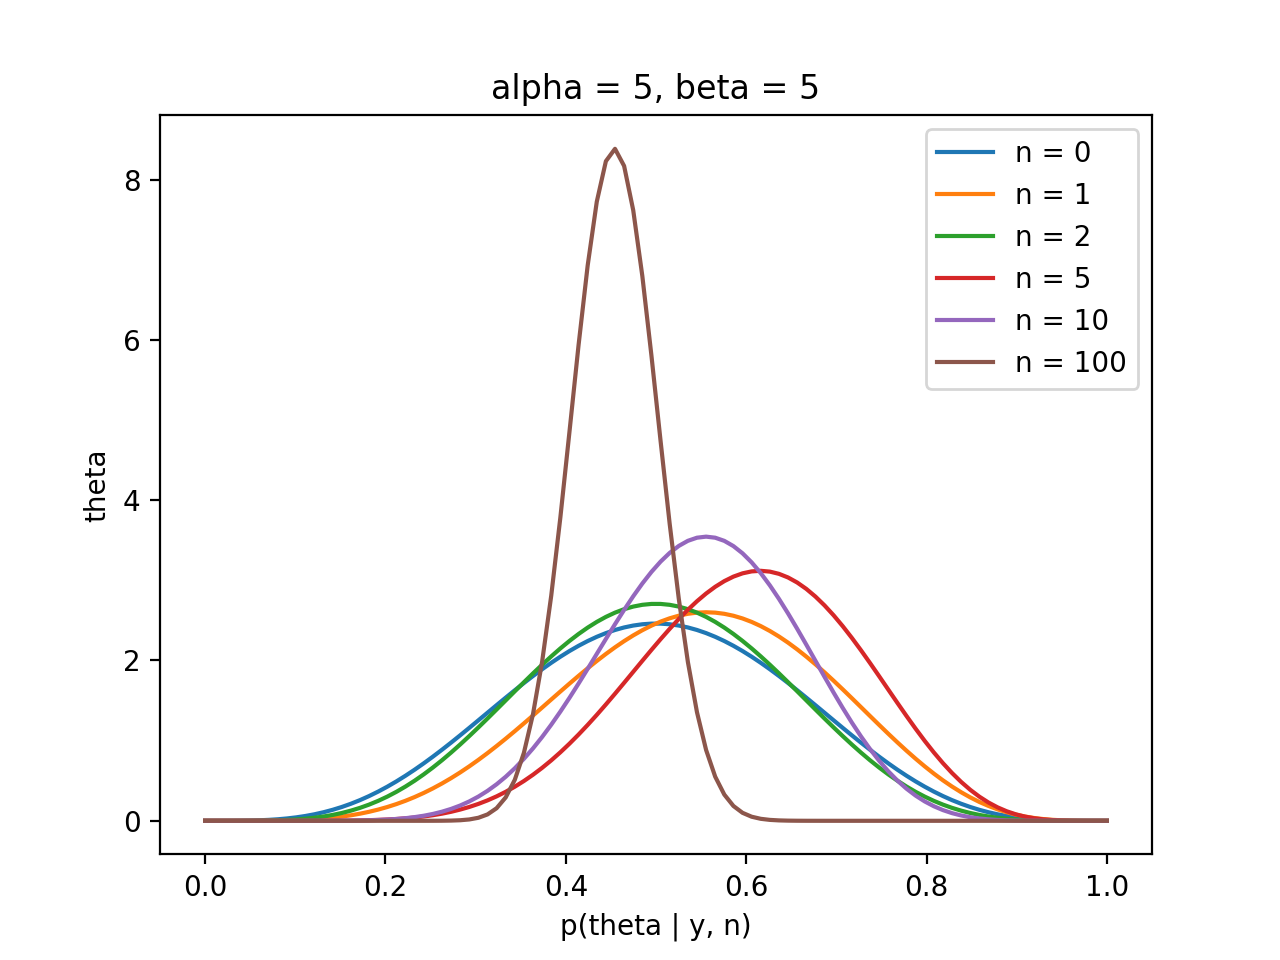
\includegraphics[width=\linewidth]{{fig/q4.3_3}.png}
  \caption*{Unbiased coin}
\endminipage\hfill
\minipage{0.4\textwidth}
    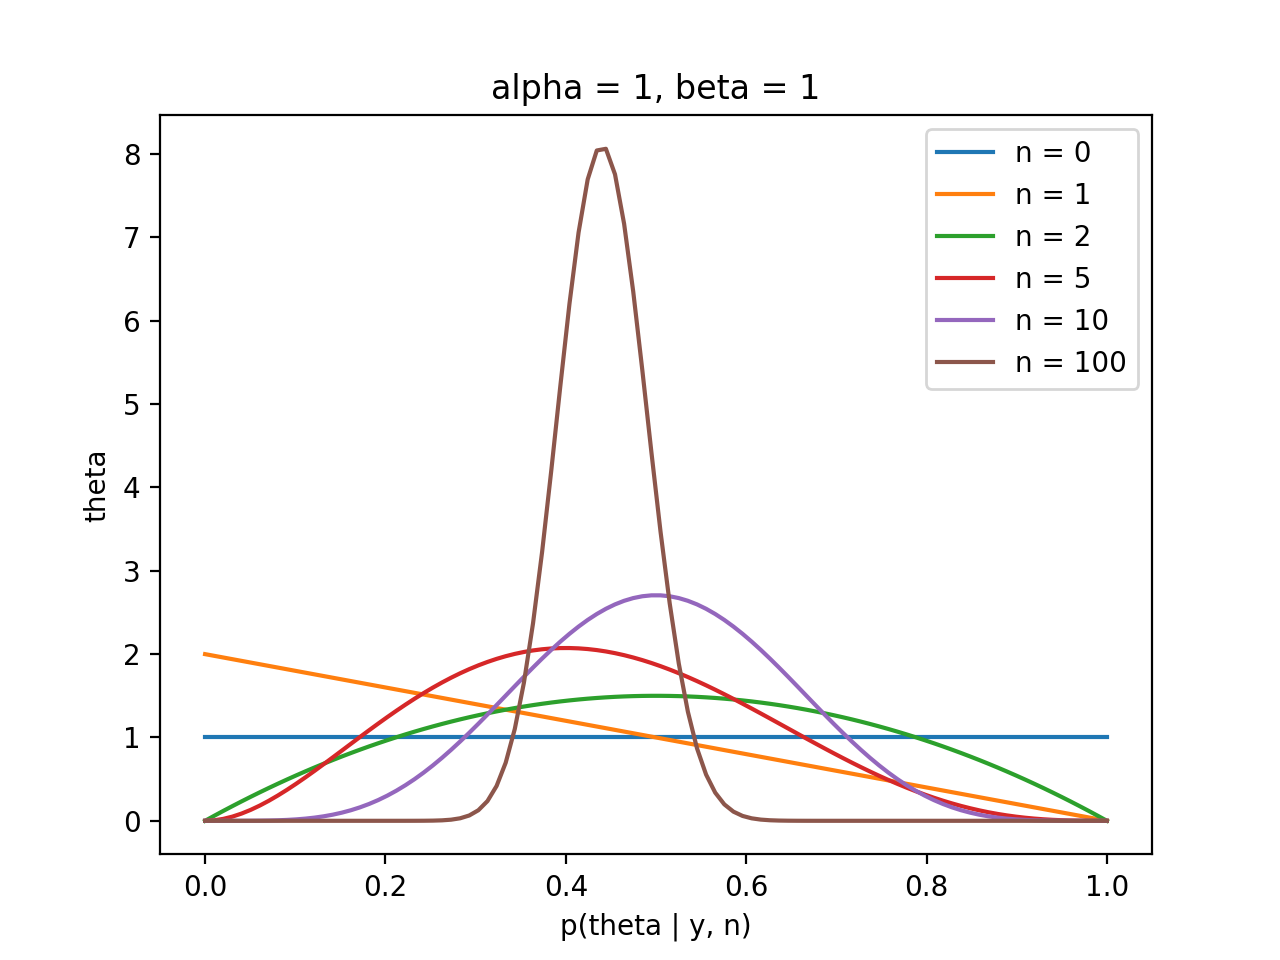
\includegraphics[width=\linewidth]{{fig/q4.3_4}.png}
    \caption*{No info coin}
\endminipage
\end{figure}


\subsection*{4.4.}

Yes, as $n$ getting large we may more info on the likelihood and therefore result in an more accurate estimation. We may confirm this by checking at $n = 100$, regardless which prior we used, the prediction came out to be unbiased and accurate (around $\theta = 0.5$).

\section*{Q5}

Please refer to \ilc{code/q5.py} for code.

\subsection*{5.1.}

Let $x$ to be the actual occurence of events per unit time, we have:

\begin{equation*}
    p(x \mid \lambda) = \frac{e^{-\lambda} \lambda^x}{x!}
\end{equation*}

Since we have $9$ events occured in a duration of $3$ seconds, we estinate $\lambda = 3$. I will also plut $\lambda = 2$ and $\lambda = 4$ as examples of ``less'' and ``greater than'' of my estimation.





\begin{figure}[H]
\minipage{0.3\textwidth}
  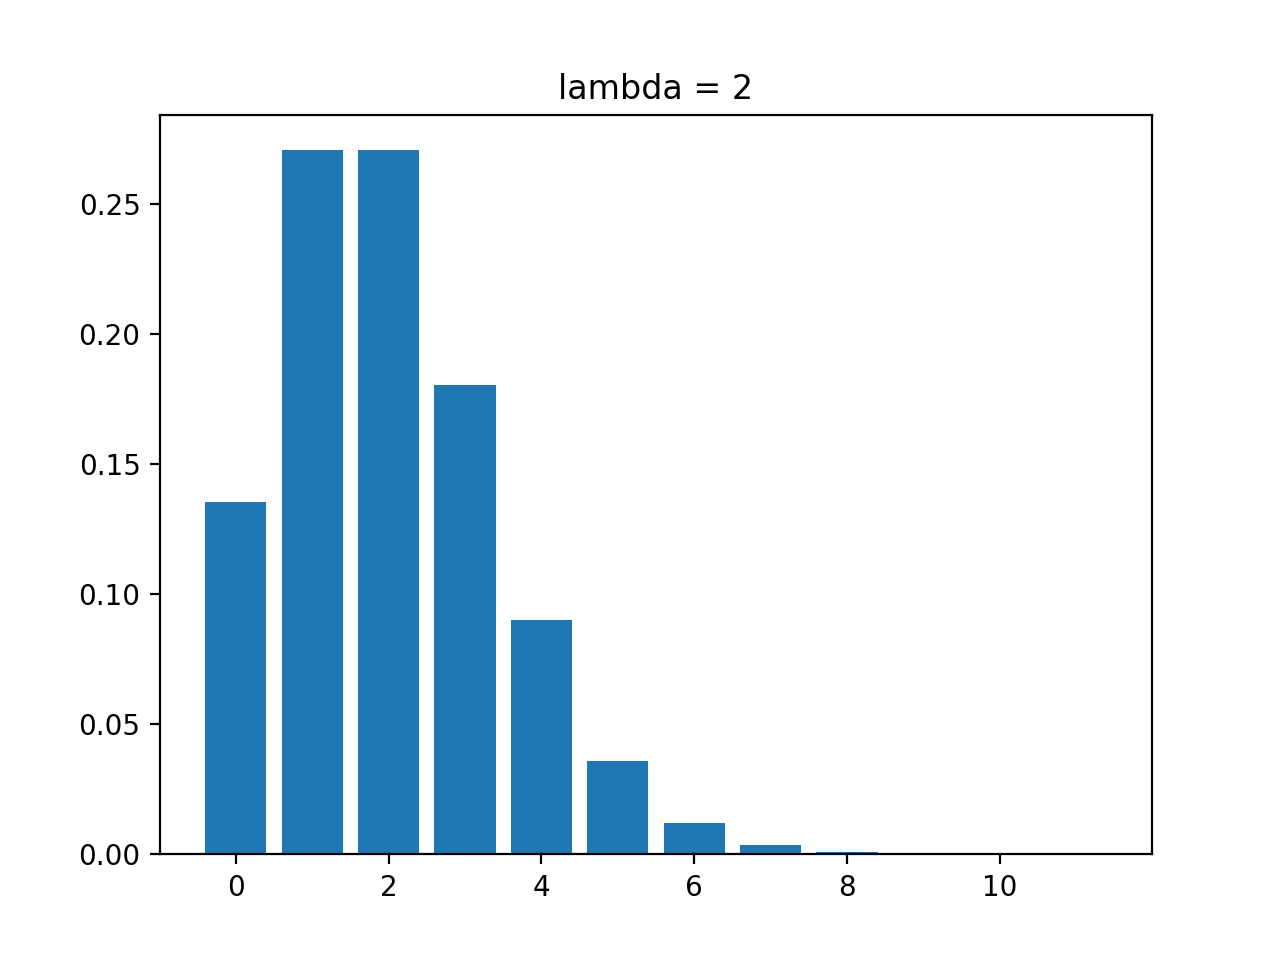
\includegraphics[width=\linewidth]{{fig/q5.1_1}.png}
  \caption*{$\lambda = 2$}
\endminipage\hfill
\minipage{0.3\textwidth}
  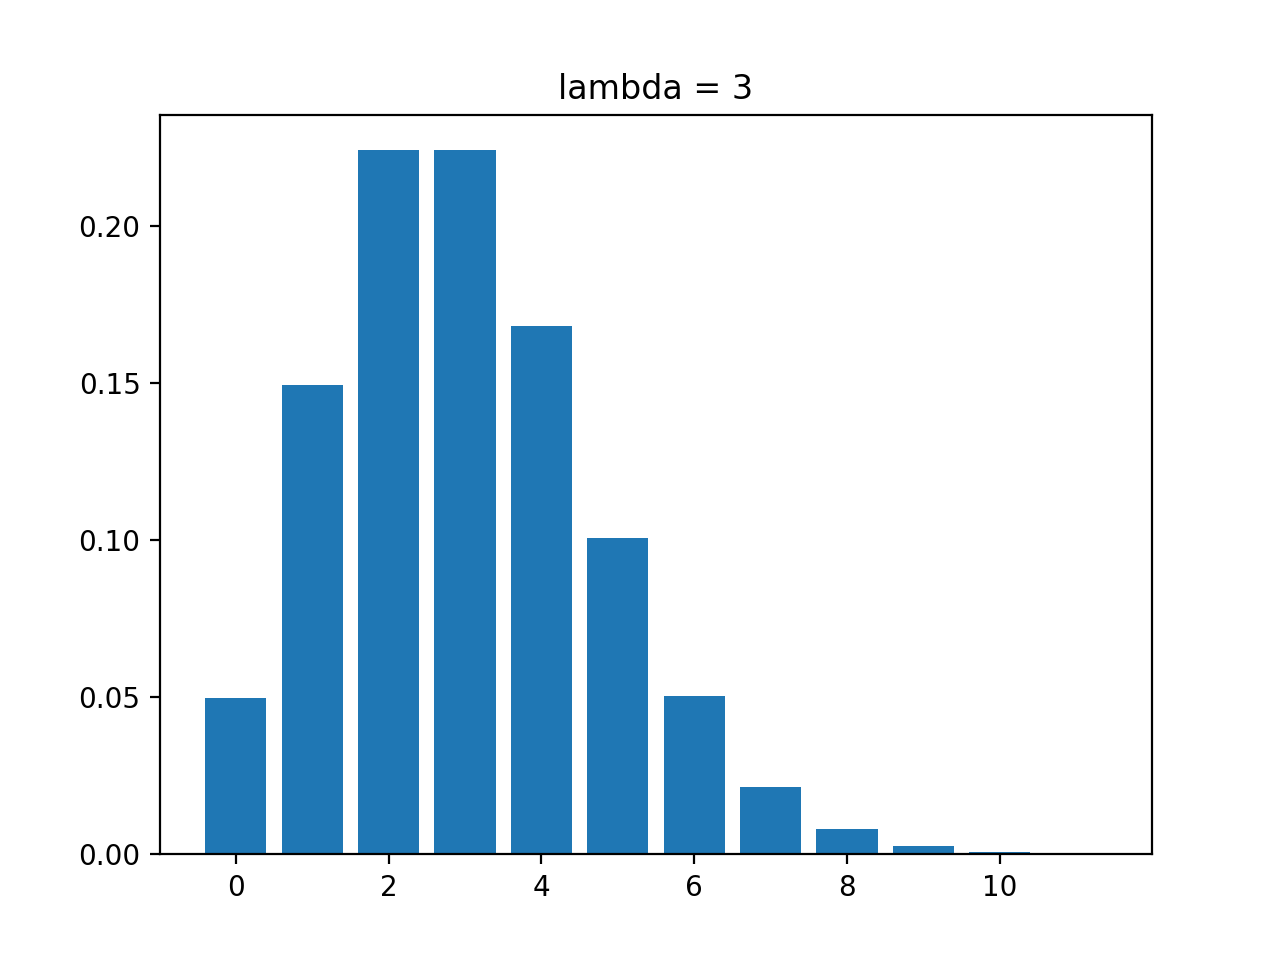
\includegraphics[width=\linewidth]{{fig/q5.1_2}.png}
  \caption*{$\lambda = 3$}
\endminipage\hfill
\minipage{0.3\textwidth}
  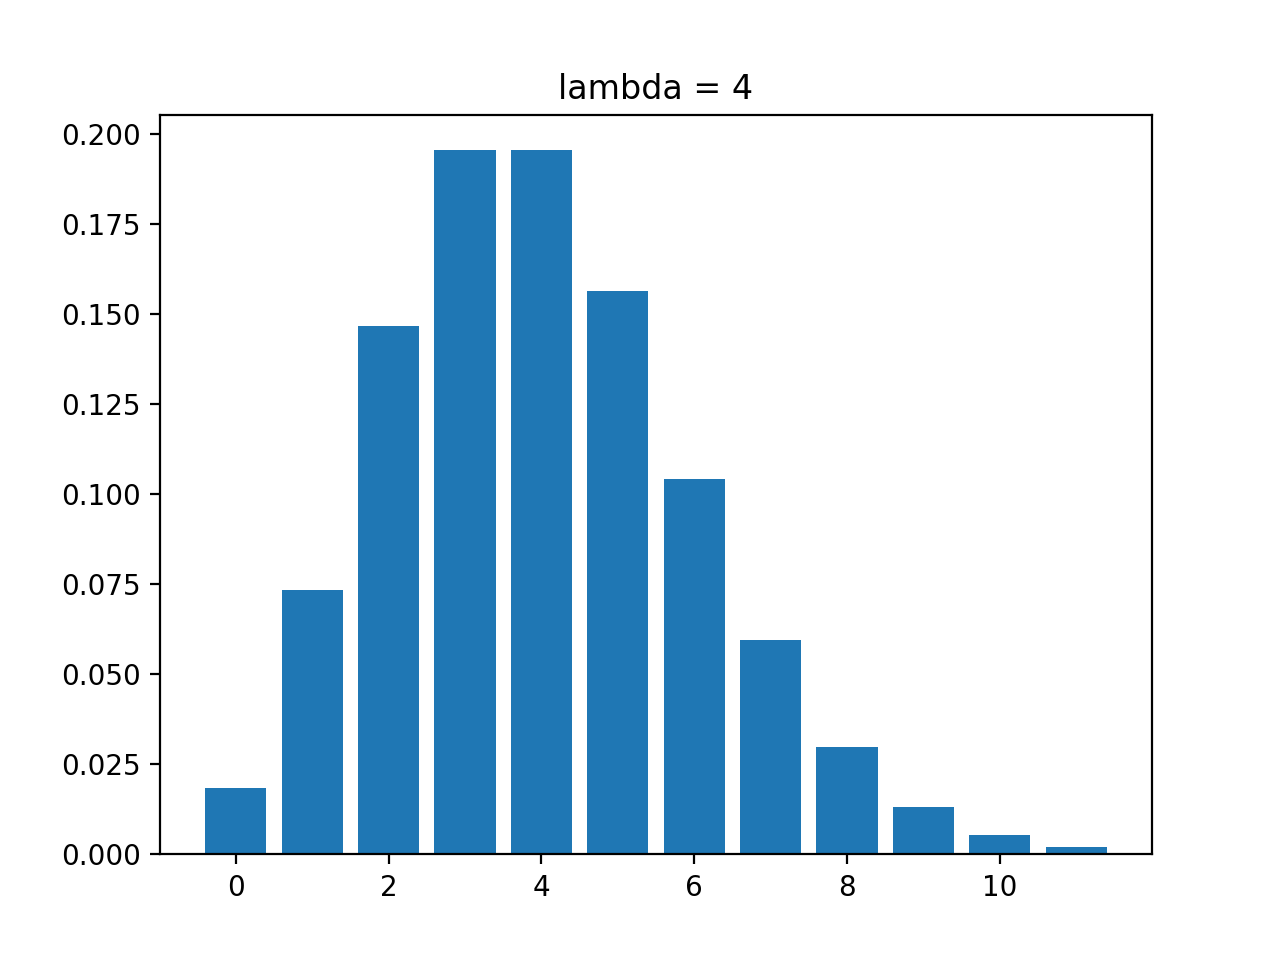
\includegraphics[width=\linewidth]{{fig/q5.1_3}.png}
  \caption*{$\lambda = 4$}
\endminipage
\end{figure}

\subsection*{5.2.}

\begin{align*}
    p(\lambda \mid n, T, \alpha, \beta) &= \frac{p(n, T \mid \lambda, \alpha, \beta) p(\lambda \mid \alpha, \beta)p(\alpha, \beta)}{p(n,T \mid \alpha, \beta)p(\alpha, \beta)}\\
    &= \frac{p(n, T \mid \lambda, \alpha, \beta) \Gamma (\lambda; \alpha, \beta)}{p(n, T \mid \alpha, \beta)}\\
    &= \frac{p(n, T \mid \lambda, \alpha, \beta) \Gamma (\lambda; \alpha, \beta)}{\int_0^{\infty}p(n, T\mid \lambda, \alpha, \beta)p(\lambda \mid \alpha, \beta) \cdot d\lambda} \\
    &= \frac{ \frac{e^{-\lambda T}(\lambda{T})^n }{n!} \cdot \Gamma(\lambda; \alpha,\beta)}{\int_0^{\infty}(\frac{e^{-\lambda{T}}(\lambda{T})^n}{n!}  \cdot \Gamma (\lambda ; \alpha,\beta))d\lambda} \\
    &= \frac{ e^{-\lambda{T}}(\lambda T )^n \cdot \lambda^{\alpha-1} e^{-\beta \lambda}}{\int_0^{\infty} e^{-\lambda (\beta + T)}(T \lambda)^n  \lambda^{\alpha-1} \cdot d\lambda}
\end{align*}

\subsection*{5.3.}

\begin{align*}
    p(\lambda \mid n, T, \alpha, \beta) &= \frac{ e^{-\lambda{T}}(\lambda T )^n \cdot \lambda^{\alpha-1} e^{-\beta \lambda}}{\int_0^{\infty} e^{-\lambda (\beta + T)}(T \lambda)^n  \lambda^{\alpha-1} \cdot d\lambda} \\
    &= \frac{\frac{(\beta + T)^{\alpha+n}T^n \lambda^{n}e^{-\lambda(\beta+T)}\lambda^{\alpha-1}}{\Gamma(a+n)}}{T^n \cdot \frac{\Gamma(a + n)}{\Gamma(a)}\frac{\beta^{\alpha}}{(T + \beta)^{a+n}}} \\
    % {T^n \int_0^{\infty} \frac{(\beta+T)^{\alpha+n}\lambda^n e^{-\lambda(\beta+T)}}{\Gamma(a+n)}d\lambda} \\
    &= \frac{(\beta+T)^{\alpha+n}\lambda^{\alpha+n-1}e^{-\lambda(\beta+T)}}{\Gamma(a+n)} \\ \\
    &= \Gamma(\lambda; \alpha+n, \beta+T)
\end{align*}

Thus, the Gamma distribution is the conjugate prior of Possion distribution with $\alpha' = \alpha + n$ and $\beta' = \beta + T$.

\subsection*{5.4.}

\begin{figure}[H]
    \centering
    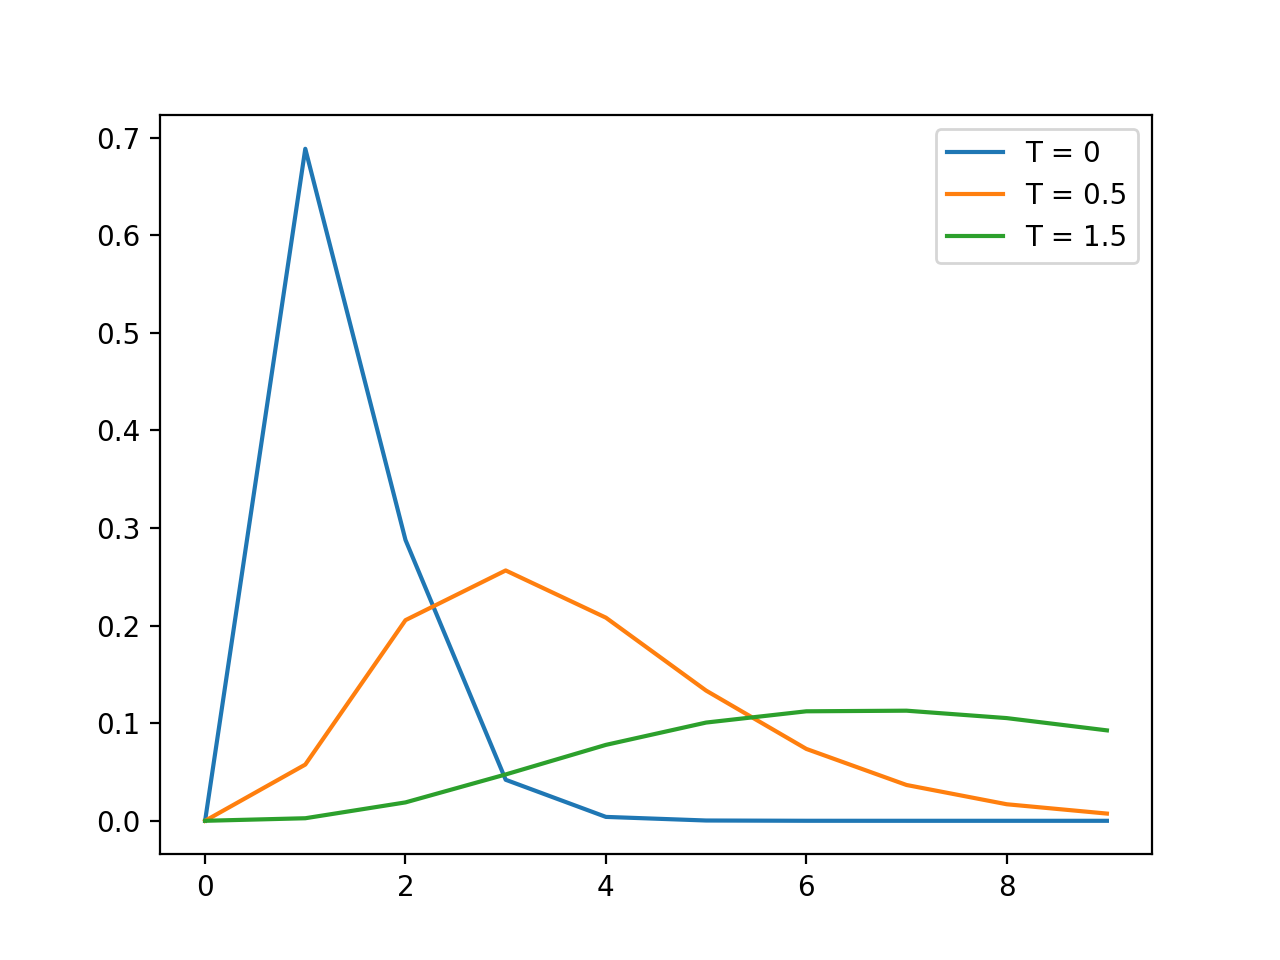
\includegraphics[width=0.6\linewidth]{{fig/q5.4}.png}
\end{figure}

Although no new event has occured, the fact that no event has occured bring in useful information to the estimation.

\section*{Q6}

\textit{The following example is altered from the book}.\newline

\noindent Assuem we have two 3-side dice to roll where we the first dice being $X \in \{1, 2, 3\}$ and $Y$ being the sum of two dices. We have the joint probability being:

\begin{table}[H]
    \centering
    \begin{tabular}{ c | c | c | c}
        \hline
        $p(x, y)$ & $X = 1$ & $X = 2$ & $X = 3$ \\
        \hline
        $Y = 2$ & 1/9 & 0 & 0 \\
        $Y = 3$ & 1/9 & 1/9 & 0 \\
        $Y = 4$ & 1/9 & 1/9 & 1/9 \\
        $Y = 5$ & 0 & 1/9 & 1/9 \\
        $Y = 6$ & 0 & 0 & 1/9 \\
    \end{tabular}
\end{table}

I capture the structure in such a way that if $y - x > 3$, the probability will be $0$ as the max roll from second dice is only $3$. If $y - x \leq 3$, this means we can only have one possible second dice outcome to match with the first dice, so the join probability will bt $(\frac{1}{3})^2 = \frac{1}{9}$.

For conditional probablity, we have $p(y | x) = \frac{p(x, y)}{x}$. But since given a certain $x$, we will have only one option, $(y - x)$, for the second dice; thus, we have $p(y | x) = \frac{1}{3}$ if such $(x, y)$ combination is at all possible. On the othe hand we have $p(x | y) = \frac{p(x, y)}{y}$. Since we only have one first-second dice combination given a possible $(x, y)$, $p(x | y) = p(x) \cdot p(\text{second dice outcome}) = \frac{1}{9}$.

For marginal probablity for $P(x)$, is it universially $\frac{1}{3}$ due to the nature of being a fair dice. But for $P(Y)$ we have:

\begin{equation*}
    P(y) = \sum_{j} P(x_j, y)
\end{equation*}

\begin{table}[H]
    \centering
    \begin{tabular}{ c | c | c | c | c | c}
        \hline
         & $Y = 2$ & $Y = 3$ & $Y = 4$ & $Y = 5$ & $Y = 6$ \\
        \hline
        $P(Y)$ & 1/9 & 2(1/9) & 3(1/9) & 2(1/9) & 1/9
    \end{tabular}
\end{table}

The intuition behind this equation is to get a certain $Y$, you must add the all possible dice combination to form such $Y$ by chances. Which means we may simply add up each row of the joint probablity table to form a table for all $P(Y)$.


\section*{Q7: Exploration}

\subsection*{Discrete Inference Problem}

I overhead the idea of ``draw a dice from a jar (of different dices) and roll it without checking the dice'' in classroom and thought it would be interesting. Although the proposed question in classroom was seemingly unsolvable, many interesting questions can be made base on this set up.\newline

\noindent Assuming we have a jar of three dices, $\{D4, D6, D8 \}$ representing a 4-, 6-, 8-side fair dice respectively. We may draw a dice from the jar, roll it, record the outcome and put it back. Say we got an output sequence of

\begin{equation*}
    \{1, 6, 3\}
\end{equation*}

What is the most likely sequence of the dice rolled?\newline


\noindent This question will be easy if the output sequence is $\{ 8, 8, 8\}$ so that we know the dice rolling sequence must be $\{D8, D8, D8 \}$ as no other dice can generate an outcome of $8$. This implies for $P(D \mid 8)$, we have $P_1(D4 \mid 8) = P(D6 \mid 8) = 0$ and $P(D8 \mid 8) = 1$

Although we can definitively tell what will $P_1(D_{\{4, 6, 8\}} \mid 1)$ be, we may infer base on the structure of the dice:

\begin{align*}
    P_1(D4 \mid 1) &= \frac{1}{4} \\
    P_1(D6 \mid 1) &= \frac{1}{6} \\
    P_1(D8 \mid 1) &= \frac{1}{8}
\end{align*}

So we may safely conclude that for the first outcome of the sequence $\{1\}$, it is most likely generated by $D4$. Similarily, for $\{1, 6\}$, we may find the dice-rolling sequence that has the maximal possibility of generating this output sequence. We already know the first dice is most likely to be $D4$, then we have
\begin{align*}
    P_2((D4 \mid 1)) &= P(D4) \cdot P(1 \mid D4) \cdot P(D4 \to D4) \cdot  \cdot P(6 \mid D4) \\
    P_2((D6 \mid 1)) &= P(D4) \cdot P(1 \mid D4) \cdot P(D4 \to D6) \cdot  \cdot P(6 \mid D6) \\
    P_2((D8 \mid 1)) &= P(D4) \cdot P(1 \mid D4) \cdot P(D4 \to D8) \cdot  \cdot P(6 \mid D8) \\
\end{align*}

In this case, we have $P_2((D6 \mid 1))$ yieling the largest probability, so the dice-rolling sequence is mostly likely to be $\{D4, D6\}$... and using the same idea we will have an answer of $\{D4, D6, D4\}$.\newline

This question is simple because we have a short output sequence to decode, and we may even simply brute force this problem by trying out every combinations. But the idea of calculating the most likely dice one by one can be extend to sequence of any length, and even with many more add on restructions like:

\begin{itemize}
    \item Not to use the same dice twice in a row: we may simply set $P(D_x \to D_x) = 0$.
    \item Got mutiple dice of same structure in the jar: we may simply $P(D_x \to D_y) = \frac{\text{left over $Dy$ dices}}{\text{all dices - number of $Dx$ dices}}$.
    \item There is uneven transition possibility between $D_x \to D_y$: we set $P(D_x \to D_x)$ accordingly.
\end{itemize}

This question will eventually become a dynamic programming problem to solve.

\subsection*{Continuous Inference Problem}



%
% I came across some interesting educational resources of Gaussian naive bayes with multiple random variables, and I thought this might be a good place to reiterate what I learned.
%
% Assume we are trying to predict weather a person loves a certain movie base on the amount of popcorn, soda pop, and candy this person consumed. We will have a 3-dimension continuous inference problem as the amount of food consumption is continuous (we also assume each food consumption distribution is Normal distribution).
%
% For visualization, let color green represents the food consumption distribution of the group who loves this movie, and color red represents the  food consumption distribution of the group who does not. The \textbf{X} mark is the person to predict as he has consumed $C = \{20, 500, 25\}$ units of popcorn, soda, and candy respectively:
%
% \begin{figure}[H]
%     \centering
%     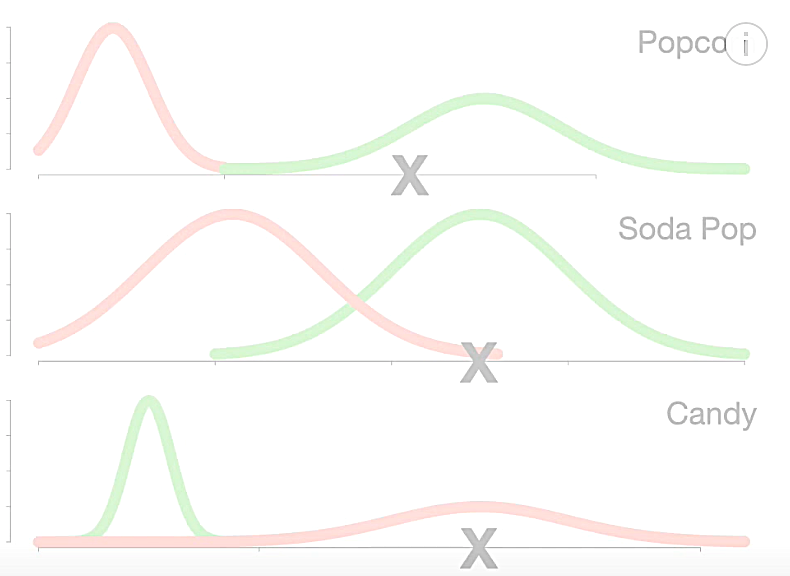
\includegraphics[width=0.6\linewidth]{{fig/q7}.png}
% \end{figure}
%
% Intuitively, we would assume this person will belong to the group who love such movie as he has consumed a lor more popcorn and soda than the group who doesn't. To form the equation, we may have:
%
% \begin{align*}
%     p(L \mid C) &= \frac{p(L) \cdot p(p = 20 \mid L) \cdot p(s = 500 \mid L) \cdot p(c = 25 \mid L)}{P(C)} \\
%     &= \frac{p(L) \cdot p(p = 20 \mid L) \cdot p(s = 500 \mid L) \cdot p(c = 25 \mid L)}{\int p(C \mid L)p(L) \cdot dL} \\
%     p(\hat{L} \mid C) &= \frac{p(\hat{L}) \cdot p(p = 20 \mid \hat{L}) \cdot p(s = 500 \mid \hat{L}) \cdot p(c = 25 \mid \hat{L})}{P(C)} \\
%     &= \frac{p(\hat{L}) \cdot p(p = 20 \mid \hat{L}) \cdot p(s = 500 \mid \hat{L}) \cdot p(c = 25 \mid \hat{L})}{\int p(C \mid \hat{L})p(\hat{L}) \cdot d \hat{L}}
% \end{align*}
%
% In this question we assumed $p(L) = p(\hat{L})$ as prior.

I will try to discuss how gramma distribution is a conmjugate prior for exponential distribution.

For $\theta \sim Gamma(\alpha, \beta)$ we have a prior of:

\begin{equation*}
    f_\Theta(\theta) = \frac{\beta^\alpha\theta^{\alpha - 1}e^{-\beta\theta}}{\Gamma(\alpha)}
\end{equation*}

It's likelihood is a exponential distribution:

\begin{equation*}
    f(X|\theta) = \theta^n e^{-\theta \sum x_i}
\end{equation*}

Now to find the posterior (likelihood times prior):

\begin{align*}
    f_{\Theta | X}(\theta | x) &\propto f_{x|\Theta}(x|\theta)\times f_\Theta(\theta) \\
    f_{\Theta | X}(\theta | x) &\propto \theta^n e^{-\theta \sum x_i} \times \frac{\beta^\alpha\theta^{\alpha - 1}e^{-\beta\theta}}{\Gamma(\alpha)} \\
    &= \theta^{n + \alpha - 1}e^{-\theta(\sum x_i + \beta)}
\end{align*}

We have a gamma distribution of $\Gamma( \alpha' = \alpha + n, \beta' = \beta + \sum x_i )$ being the conjugate prior.

\end{document}

